\documentclass[letterpaper,12pt]{article}

\usepackage{tabularx} % extra features for tabular environment
\usepackage{amsmath}  % improve math presentation
\usepackage{amssymb}
\usepackage{multirow}
\usepackage{xcolor}
\usepackage{gensymb}
\usepackage{appendix}
\usepackage{verbatim}
\usepackage{bigints}

\usepackage{mathtools}
\usepackage{gensymb}
\usepackage{float}
\usepackage{listings}
\usepackage[export]{adjustbox}
\usepackage[super]{nth}
\usepackage{graphicx} % takes care of graphic including machinery
\usepackage[margin=1in,letterpaper]{geometry} % decreases margins
\usepackage{cite} % takes care of citations
\usepackage[final]{hyperref} % adds hyper links inside the generated pdf file

\newcommand*{\tran}{^{\mkern-1.5mu\mathsf{T}}}
\DeclarePairedDelimiter\ceil{\lceil}{\rceil}
\DeclarePairedDelimiter\floor{\lfloor}{\rfloor}
\hypersetup{
    colorlinks=false,       % false: boxed links; true: colored links
    linkcolor=blue,        % color of internal links
    citecolor=blue,        % color of links to bibliography
    filecolor=magenta,     % color of file links
    urlcolor=blue         
}
%++++++++++++++++++++++++++++++++++++++++++++++++++++++++++++++++++++++++++++++++



%++++++++++++++++++++++++++++++++++++++++++++++++++++++++++++++++++++++++++++++++
% Start modifying the labwork number, your team number and the name and METU id
% of your group members.
\newcommand{\reporttitle}{Solution Set 7}
\newcommand{\reportauthor}{ Volkan Aydıngül (Id: 0075359 )\\
                            }
                            % If any teammate does not help to write this report,
                            % you may not write his/her name here.
%++++++++++++++++++++++++++++++++++++++++++++++++++++++++++++++++++++++++++++++++



%++++++++++++++++++++++++++++++++++++++++++++++++++++++++++++++++++++++++++++++++
% DO NOT MODIFY THIS SECTION
\begin{document}
\begin{titlepage}
\newcommand{\HRule}{\rule{0.7\linewidth}{0.5mm}}
\begin{center} % Center remainder of the page
%	LOGO SECTION

\includegraphics[width = 8cm]{figures/koc_logo.png}

%	HEADING SECTIONS
\textsc{\Large PHYS 514 - Computational Physics}\\[1.5cm] 
%	TITLE SECTION
\HRule \\[0.6cm]
{ \huge \bfseries \reporttitle}\\ % Title of your document
\HRule \\[1.5cm]
\end{center}
\vspace{2cm}
%	AUTHOR SECTION
\begin{flushleft} \large
\textit{Author:}\\
\reportauthor% Your name
\end{flushleft}
\vspace{2cm}
\makeatletter
Date: \@date 
\vfill % Fill the rest of the page with whitespace
\makeatother
\end{titlepage}
%++++++++++++++++++++++++++++++++++++++++++++++++++++++++++++++++++++++++++++++++




\tableofcontents
\newpage





%\begin{figure}[H] 
%   \centering \includegraphics[width=\columnwidth]{figures/figure.png}           
%                \caption{Caption}                
%                   \label{fig:label}
%   \end{figure}


\section{Problem XXI}
\subsection{Construction of Symmetric Second Derivative Matrix for Neumann Boundary Condition}
\paragraph{} In the problem construction, the following information is given:
\begin{itemize}
    \item Neumann boundary condition, such that $y'(a) = 0$ and  $y'(b) = 0$
    \item Discretization scheme is such that $x_i = a + \left(i + \frac{1}{2}\right)\frac{b-a}{N}$ for $i = 0, 1, \dots, N-1$
\end{itemize}

\paragraph{} The first thing that should be done is to observe the behavior of the start and end points. Because, the intermediate points have always the same structure. For example, the following relation can be observed for $y''_{0}$ and $y''_{N-1}$:

\begin{equation}
    \label{eq:y0dd}
    y''_0 = \frac{y_1 -2y_0+y_{-1}}{h^2}
\end{equation}

\begin{equation}
    \label{eq:yNdd}
    y''_{N-1} = \frac{y_{N} -2y_{N-1}+y_{N-2}}{h^2}
\end{equation}

The fact that the $y_{-1}$ and $y_{N}$ are unknown can be immediately observed. To be able to have an idea about the $y_{-1}$ and $y_{N}$, one can easily incorporate the information of the boundary conditions. Since it is known that the $x_{-\frac{1}{2}} = a$ and $x_{N-\frac{1}{2}} = b$, the following relations can be hold:

\begin{equation*}
    y'_{-\frac{1}{2}} = \frac{y_{-\frac{1}{2}} - y_{-1}}{\frac{h}{2}} = 0
\end{equation*}

\begin{equation*}
    y'_{-\frac{1}{2}} = \frac{y_{-\frac{1}{2}} - y_{0}}{\frac{h}{2}} = 0
\end{equation*}

\begin{equation*}
    y_{-\frac{1}{2}} = y_{-1}
\end{equation*}

\begin{equation*}
    y_{-\frac{1}{2}} = y_{0}
\end{equation*}

\begin{equation*}
    \boxed{y_{-1} = y_{0}}
\end{equation*}

\paragraph{} Similarly for the end point, the following relation can be hold:

\begin{equation*}
    y'_{N-\frac{1}{2}} = \frac{y_{N-\frac{1}{2}} - y_{N-1}}{\frac{h}{2}} = 0
\end{equation*}

\begin{equation*}
    y'_{N-\frac{1}{2}} = \frac{y_{N-\frac{1}{2}} - y_{N}}{\frac{h}{2}} = 0
\end{equation*}

\begin{equation*}
    y_{N-\frac{1}{2}} = y_{N-1}
\end{equation*}

\begin{equation*}
    y_{N-\frac{1}{2}} = y_{N}
\end{equation*}

\begin{equation*}
    \boxed{y_{N-1} = y_{N}}
\end{equation*}


\paragraph{} Now, it is time to turn back to the \eqref{eq:y0dd} and \eqref{eq:yNdd}. That is, \eqref{eq:y0dd} and \eqref{eq:yNdd} can be written in the following form:

\begin{equation*}
    y''_0 = \frac{y_1 -2y_0+y_{0}}{h^2} = \frac{y_1 - y_{0}}{h^2}
\end{equation*}

\begin{equation*}
y''_{N-1} = \frac{y_{N-1} -2y_{N-1}+y_{N-2}}{h^2} = \frac{-y_{N-1}+y_{N-2}}{h^2}
\end{equation*}

\paragraph{} Moreover, the second derivative for the other data point can be easily expressed as in below form:
\begin{equation*}
    \label{eq:gendd}
    y''_k = \frac{y_{k+1} -2y_k + y_{k-1}}{h^2}
\end{equation*}

for $k = 1,2,\dots, N-2$

\paragraph{} Using all of the aforementioned information here, one can construct the second derivative matrix as in the following way:

\begin{equation*}
    \frac{d^2}{dx^2} \rightarrow \frac{1}{h^2}\begin{bmatrix}
        -1 & 1 & 0 & 0 & \hdots\\
        1  & -2 & 1 & 0 & 0 &\hdots\\
        0  & 1 & -2 & 1 & 0 & 0 &\hdots \\
        0  & 0 & 1 & -2 & 1 & 0 & 0 &\hdots\\
           &   & \ddots  & \ddots   & \ddots  \\ 
           \\
           \\
           \\
        0 & 0 & 0 & 0 &  & \hdots  &   &  1 & -2 & 1 \\ 
        0 & 0 & 0 & 0 &  & \hdots  &   &  0 & 1 & -1 \\   
    \end{bmatrix}
\begin{comment}
    \begin{bmatrix}
        y_0 \\
        y_1 \\
        y_2 \\
        \\
        \vdots \\
        \vdots \\
        \\
        y_{N-3} \\
        y_{N-2} \\
        y_{N-1} \\
                
    \end{bmatrix} = 
    \begin{bmatrix}
        \rho_0 \\
        \rho_1 \\
        \rho_2 \\
        \\
        \vdots \\
        \vdots \\
        \\
        \rho_{N-3} \\
        \rho_{N-2} \\
        \rho_{N-1} \\
    \end{bmatrix}
\end{comment}
\end{equation*}

\paragraph{} \textit{Voila! It is simétrico.}

\subsection{Construction of Second Derivative Matrix for Robin Boundary Condition}

\paragraph{} In this \textit{Hermitian} matrix derivation, the non-symmetric construction will be the chosen path. Therefore, the following sampling scheme will be used:
\begin{equation*}
    x_i = a + i\frac{b-a}{N}
\end{equation*}
for $i = 0, 1, \dots, N$

\paragraph{} In this case, still, \eqref{eq:gendd} preserves its generality for $k = 1, 2, \dots, N-1$. However, again, the behavior at the end and start points should be observed in a detailed way. One can investigate the second derivative terms at the tips with the help of the following relation:

\begin{equation}
    \label{eq:y0dd1}
    y''_0 = \frac{y_1 -2y_0+y_{-1}}{h^2}
\end{equation}

\begin{equation}
    \label{eq:yNdd1}
    y''_{N} = \frac{y_{N+1} -2y_{N}+y_{N-1}}{h^2}
\end{equation}

Now, to be able to have an idea of the unknown points, i.e. $y_{-1}$ and $y_{N+1}$, one should incorporate the knowledge of the boundary conditions. In this case, the Robin boundary conditions are subject to the problem, and its general structure can be observed below:

\begin{equation*}
    \alpha_1 y(a) + \alpha_2 y'(a) = 0 
\end{equation*}

\begin{equation*}
    \beta_1 y(b) + \beta_2 y'(b) = 0
\end{equation*}


\paragraph{} Now, it is time to write the boundary conditions in disretisized form to obtain a expression for unknown. To illustrate, the disretisized version of the boundary condition at the starting point can be observed below:

\begin{equation*}
    \alpha_1 y_0 + \alpha_2 \left(\frac{y_0 - y_{-1}}{h}\right) = 0
\end{equation*}

\begin{equation*}
    \alpha_1 y_0 + \frac{\alpha_2 y_0}{h} = \frac{\alpha_2 y_{-1}}{h}
\end{equation*}

\paragraph{} Reasonably, $y_{-1}$ can written in the following form:

\begin{equation*}
    y_{-1} = y_0 \left(\frac{\alpha_1h}{\alpha_2} + 1\right)
\end{equation*}

\paragraph{} Finally, \eqref{eq:y0dd1} can be rewritten in terms of the known variables:

\begin{equation*}
    y''_0 = \frac{ y_1 - 2y_0 +  y_0 \left(\frac{\alpha_1h}{\alpha_2} + 1\right)}{h^2}
\end{equation*}

\begin{equation*}
    y''_0 = \frac{ y_1 +  y_0 \left(\frac{\alpha_1h}{\alpha_2}  1\right)}{h^2}
\end{equation*}

\paragraph{} In the same way, \eqref{eq:yNdd1} can be rewritten in terms of the known variables:

\begin{equation*}
    y''_N = \frac{y_N \left(\frac{\beta_1h}{\beta_2} - 1\right)+y_{N-1}}{h^2}
\end{equation*}

\paragraph{} Finally, one can easily the second derivative matrix by making use of the aforementioned informations:
\begin{equation*}
    \frac{d^2}{dx^2} \rightarrow \frac{1}{h^2}\begin{bmatrix}
        \left(\frac{\alpha_1h}{\alpha_2} + 1\right) & 1 & 0 & 0 & \hdots\\
        1  & -2 & 1 & 0 & 0 &\hdots\\
        0  & 1 & -2 & 1 & 0 & 0 &\hdots \\
        0  & 0 & 1 & -2 & 1 & 0 & 0 &\hdots\\
           &   & \ddots  & \ddots   & \ddots  \\ 
           \\
           \\
           \\
        0 & 0 & 0 & 0 &  & \hdots  &   &  1 & -2 & 1 \\ 
        0 & 0 & 0 & 0 &  & \hdots  &   &  0 & 1 & \left(\frac{\beta_1h}{\beta_2} - 1\right) \\   
    \end{bmatrix}
\end{equation*}

\subsection{Wave Equation Solution}
\subsubsection{Dirichlet Boundary Condition - Smapling Point Experiment}


\paragraph{} From Figure \ref{fig:1_8_Standart_Eigenvalue_Solver_d_eigenvector} to Figure \ref{fig:1_50_Standart_Eigenvalue_Solver_d_eigenvector}, the effect of the number of sampling points on the accuracy of the numerical solution can be observed. In these sampling point experiments, the \textit{Root Mean Squarred Error (RMSE)} is used as an error metric. Moreover, since the eigenvectors/eigenfunctions are not calculated in an absolute manner, it is normal to observe $180 \; degree$ phase shift in some solution. To be able to eliminate this ambiguity, the \textit{RMSE} error is calculated in an absolute manner. 

\paragraph{} In Figure \ref{fig:1_8_Standart_Eigenvalue_Solver_d_eigenvector}, the large error due to the few number of sampling points can be observed. At the same time, from Figure \ref{fig:1_10_Standart_Eigenvalue_Solver_d_eigenvector} to Figure \ref{fig:1_50_Standart_Eigenvalue_Solver_d_eigenvector}, it can be observed that as the number of sampling point increase, the error rate is highly tended to decrease. 

\paragraph{} As a final note, for the number of sampling points, $n = 40$ can be implemented as a baseline point in this problem.


\begin{figure}[H]
\centerline{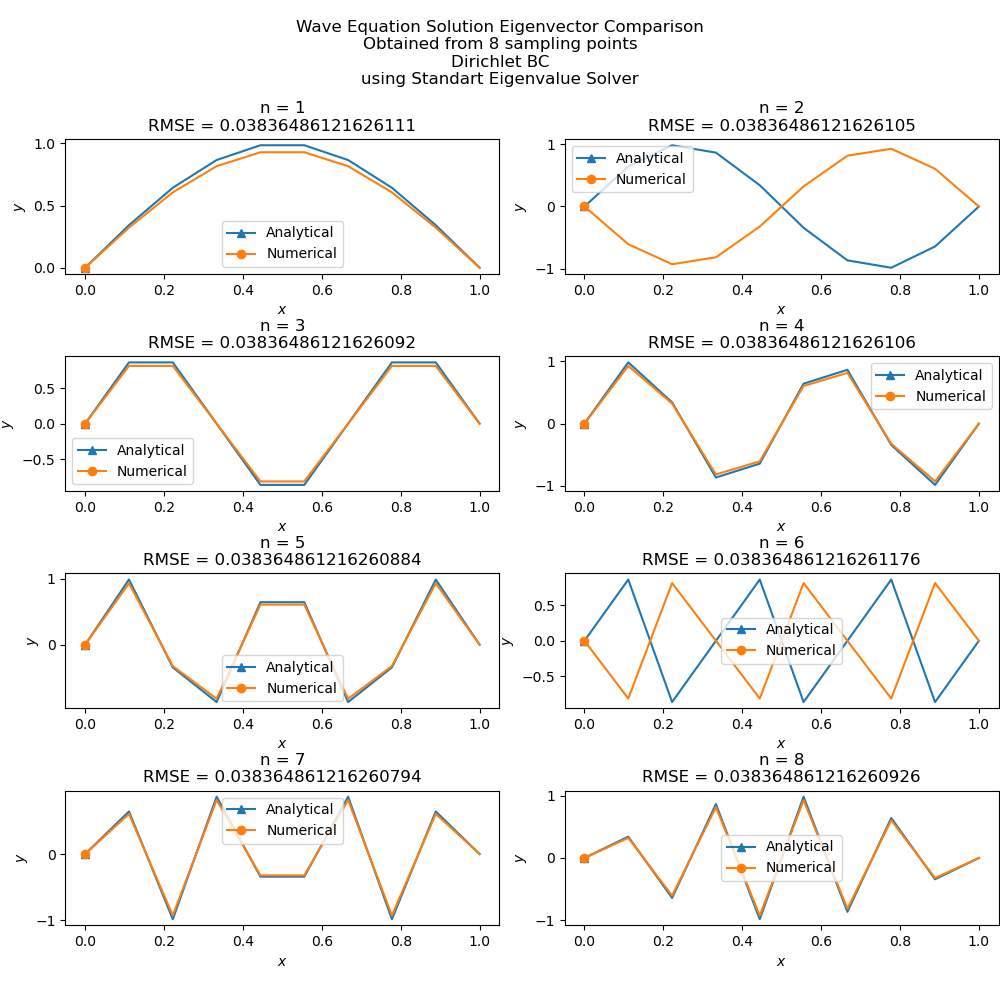
\includegraphics[width=\linewidth]{figures/1_8_Standart_Eigenvalue_Solver_d_eigenvector.png}}
\caption{Wave Equation Solution Eigenvectors - 8 Sampling Points - Standart Eigenvalue Solver - Dirichlet BC}
\label{fig:1_8_Standart_Eigenvalue_Solver_d_eigenvector}
\end{figure}

\begin{figure}[H]
\centerline{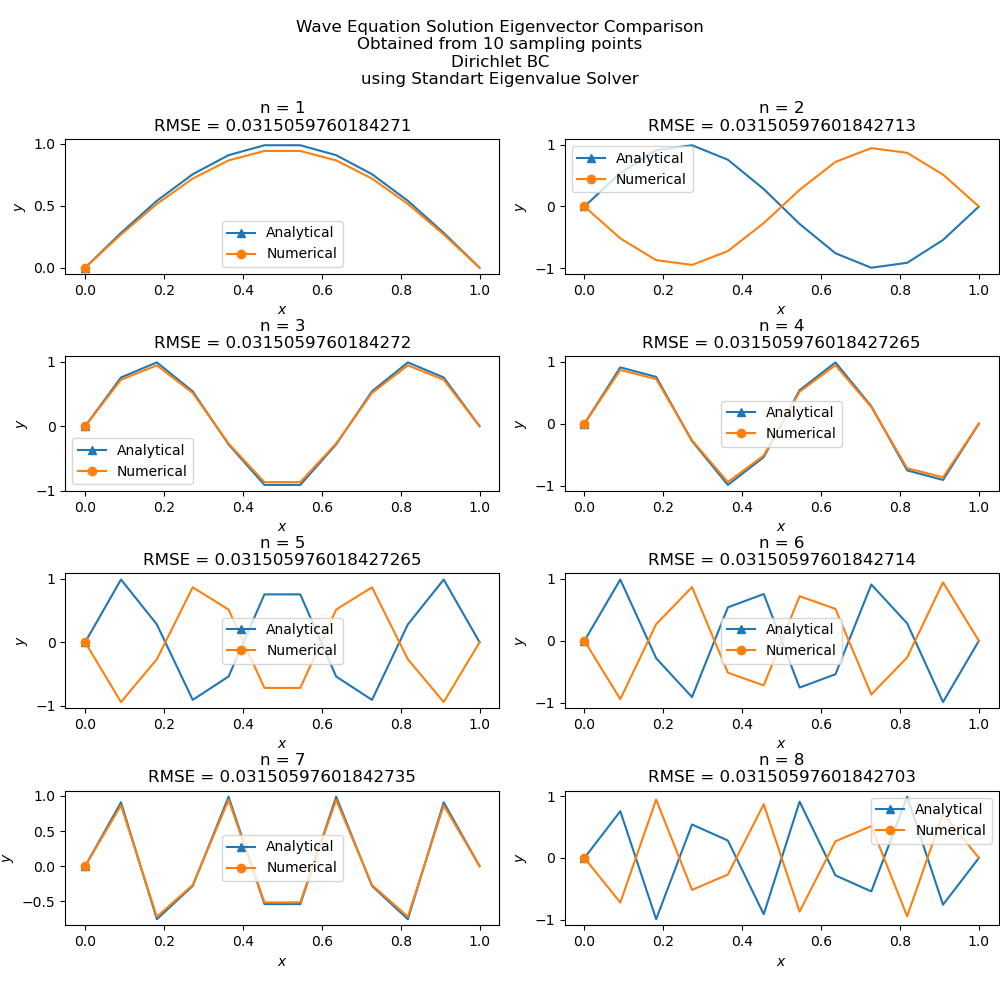
\includegraphics[width=\linewidth]{figures/1_10_Standart_Eigenvalue_Solver_d_eigenvector.png}}
\caption{Wave Equation Solution Eigenvectors - 10 Sampling Points - Standart Eigenvalue Solver - Dirichlet BC}
\label{fig:1_10_Standart_Eigenvalue_Solver_d_eigenvector}
\end{figure}

\begin{figure}[H]
\centerline{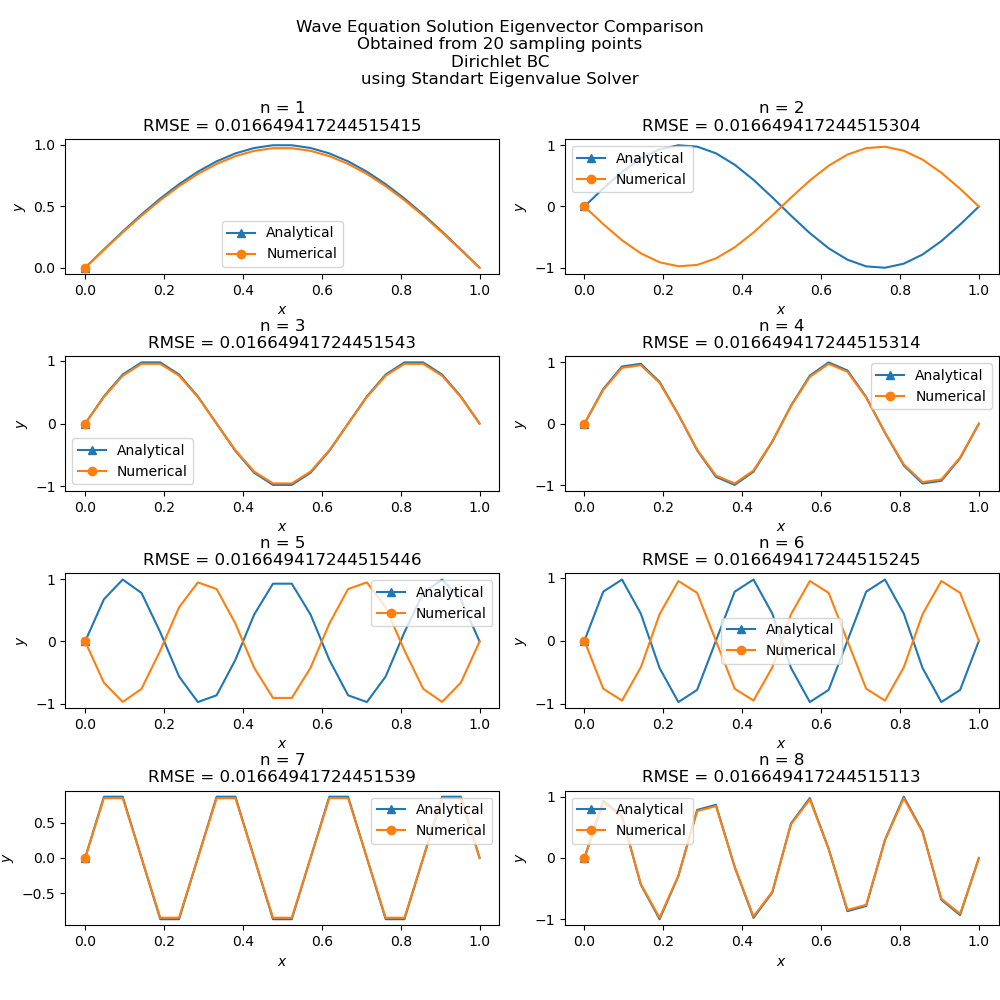
\includegraphics[width=\linewidth]{figures/1_20_Standart_Eigenvalue_Solver_d_eigenvector.png}}
\caption{Wave Equation Solution Eigenvectors - 20 Sampling Points - Standart Eigenvalue Solver - Dirichlet BC}
\label{fig:1_20_Standart_Eigenvalue_Solver_d_eigenvector}
\end{figure}

\begin{figure}[H]
\centerline{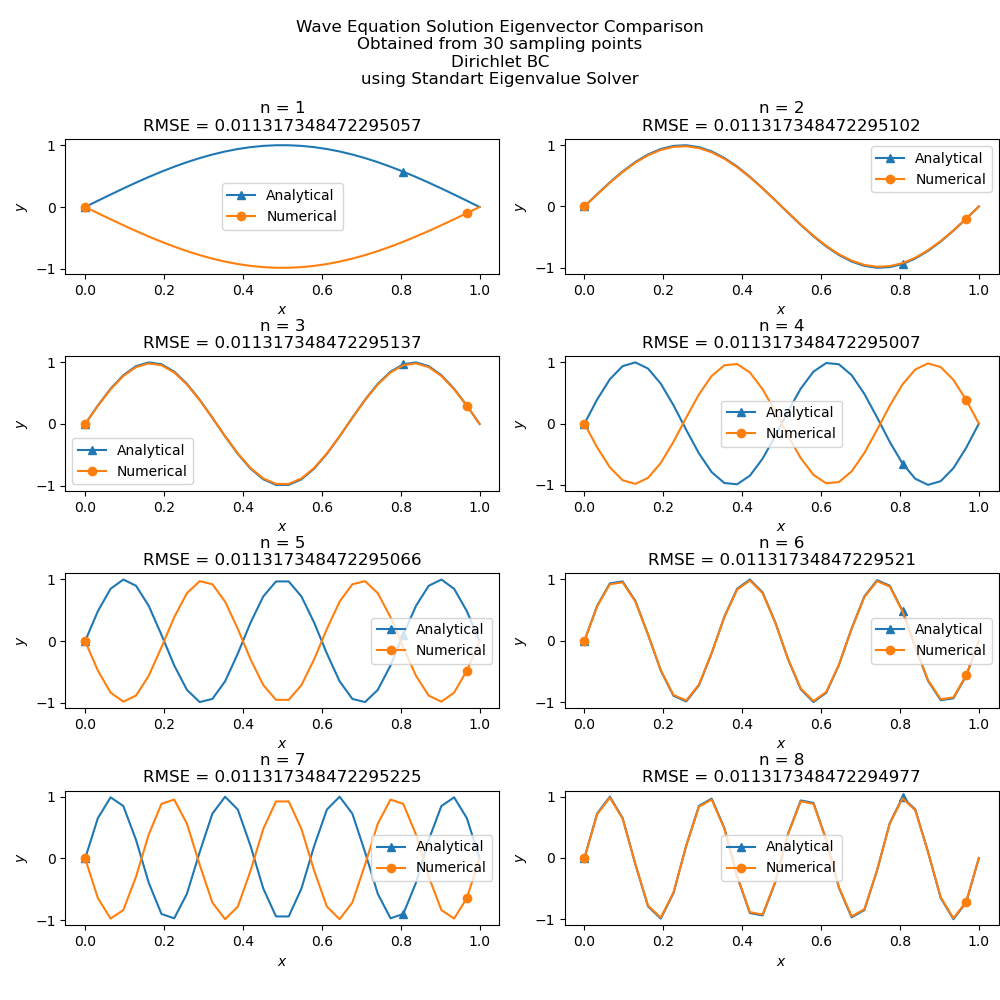
\includegraphics[width=\linewidth]{figures/1_30_Standart_Eigenvalue_Solver_d_eigenvector.png}}
\caption{Wave Equation Solution Eigenvectors - 30 Sampling Points - Standart Eigenvalue Solver - Dirichlet BC}
\label{fig:1_30_Standart_Eigenvalue_Solver_d_eigenvector}
\end{figure}

\begin{figure}[H]
\centerline{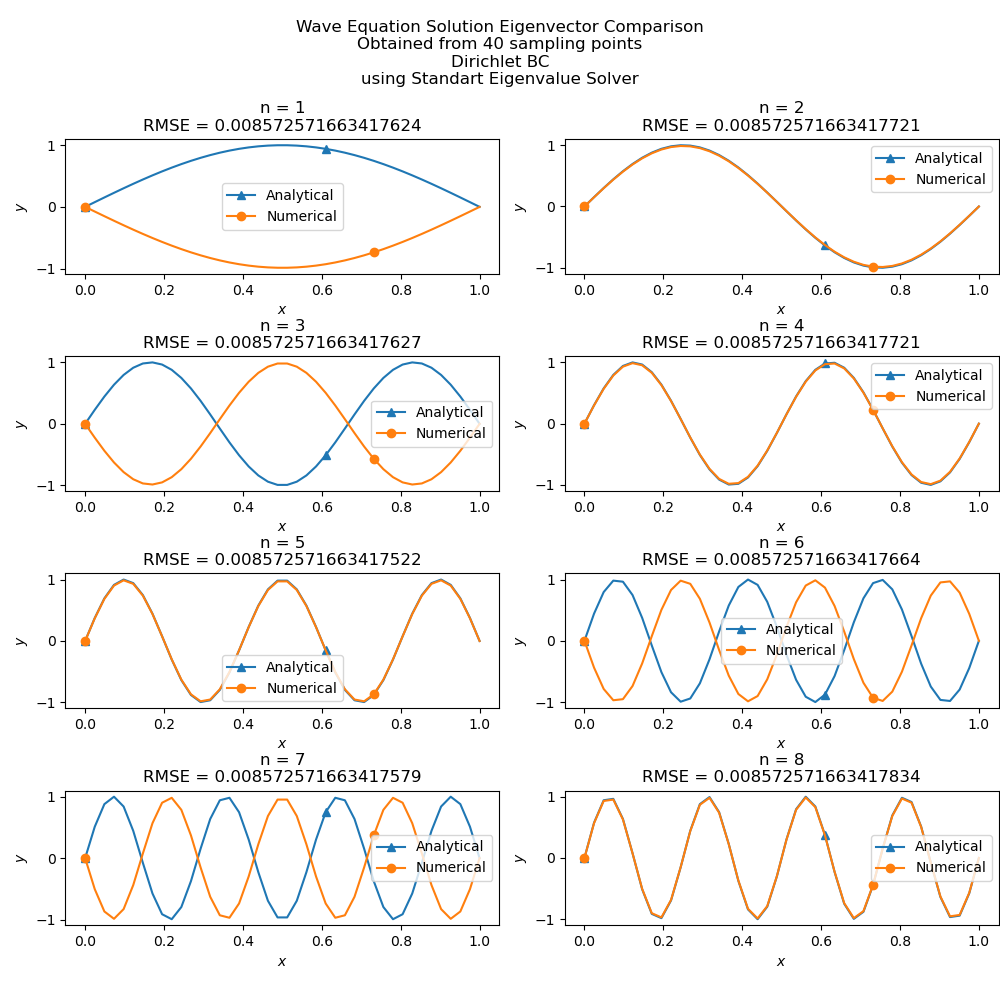
\includegraphics[width=\linewidth]{figures/1_40_Standart_Eigenvalue_Solver_d_eigenvector.png}}
\caption{Wave Equation Solution Eigenvectors - 40 Sampling Points - Standart Eigenvalue Solver - Dirichlet BC}
\label{fig:1_40_Standart_Eigenvalue_Solver_d_eigenvector}
\end{figure}

\begin{figure}[H]
\centerline{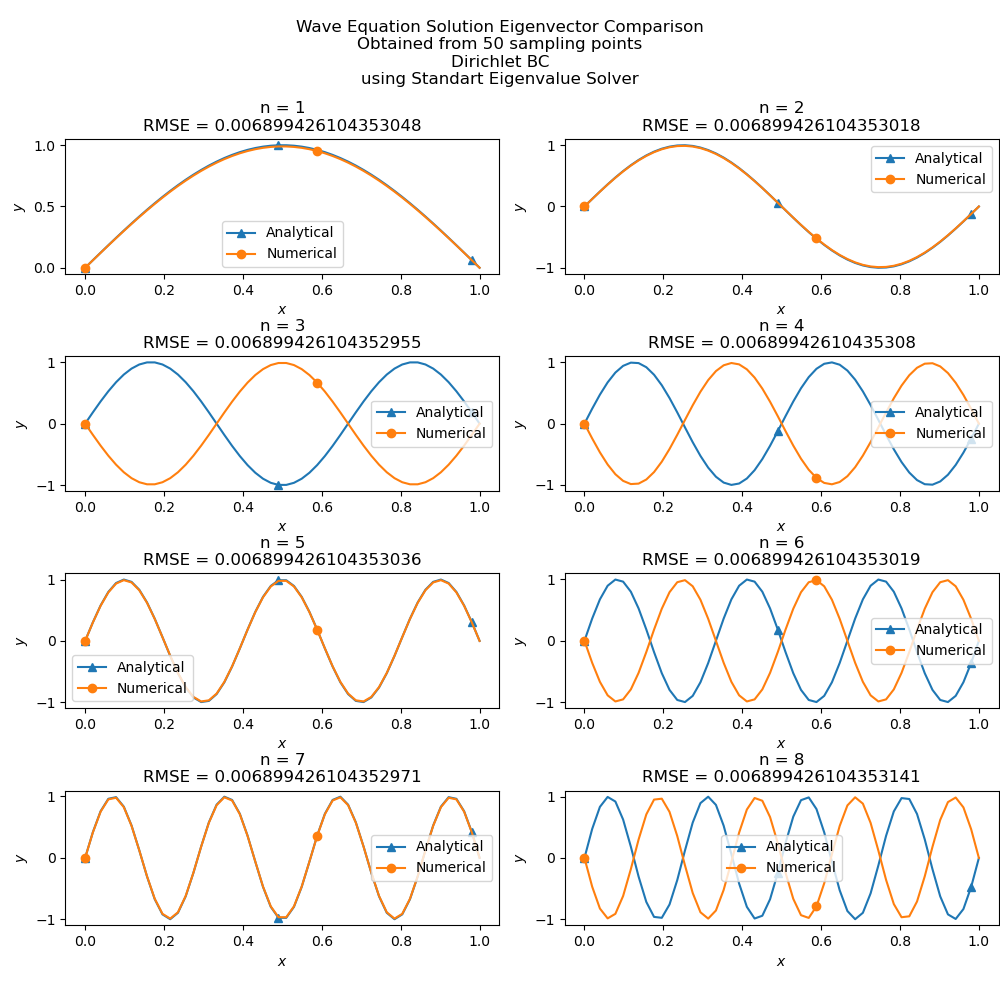
\includegraphics[width=\linewidth]{figures/1_50_Standart_Eigenvalue_Solver_d_eigenvector.png}}
\caption{Wave Equation Solution Eigenvectors - 50 Sampling Points - Standart Eigenvalue Solver - Dirichlet BC}
\label{fig:1_50_Standart_Eigenvalue_Solver_d_eigenvector}
\end{figure}


\begin{figure}[H]
\centerline{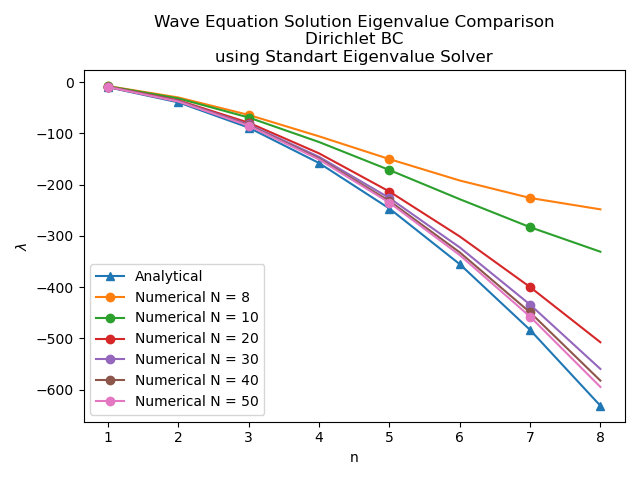
\includegraphics[width=\linewidth]{figures/1_Standart_Eigenvalue_Solver_d_eigenvalue.png}}
\caption{Wave Equation Solution Eigenvalues - Standart Eigenvalue Solver - Dirichlet BC}
\label{fig:1_Standart_Eigenvalue_Solver_d_eigenvalue}
\end{figure}

\paragraph{} Finally, the effect of the number of sampling points on the accuracy of the approximation can be observed in Figure \ref{fig:1_Standart_Eigenvalue_Solver_d_eigenvalue} more clearly. The proximity of the numerical solution to the analytical solution is a good metric to evaluate the accuracy.
    
\subsubsection{Dirichlet Boundary Condition - Eigenvalue Solver Experiment}

\paragraph{} From Figure \ref{fig:2_40_Tridiagonal_Toeplitz_Eigenvalue_Solver_d_eigenvector} to Figure \ref{fig:2_40_Symmetric_Eigenvalue_Solver_d_eigenvector}, the effect of eigenvalue solver type on the accuracy of the numerical solution can be observed. Regarding the error calcuations, the same procedure can be applicable, also, in here.

\paragraph{}From Figure \ref{fig:2_40_Tridiagonal_Toeplitz_Eigenvalue_Solver_d_eigenvector} to Figure \ref{fig:2_40_Symmetric_Eigenvalue_Solver_d_eigenvector}, it can be easily observed that the type of the eigenvalue solver does not affect the accuracy in a much serious way. However, it should be noted that the type of the eigenvalue problem solver can be distinctive factor when the speed is the issue, which will be covered in the Section \ref{sec:speed}.


\begin{figure}[H]
\centerline{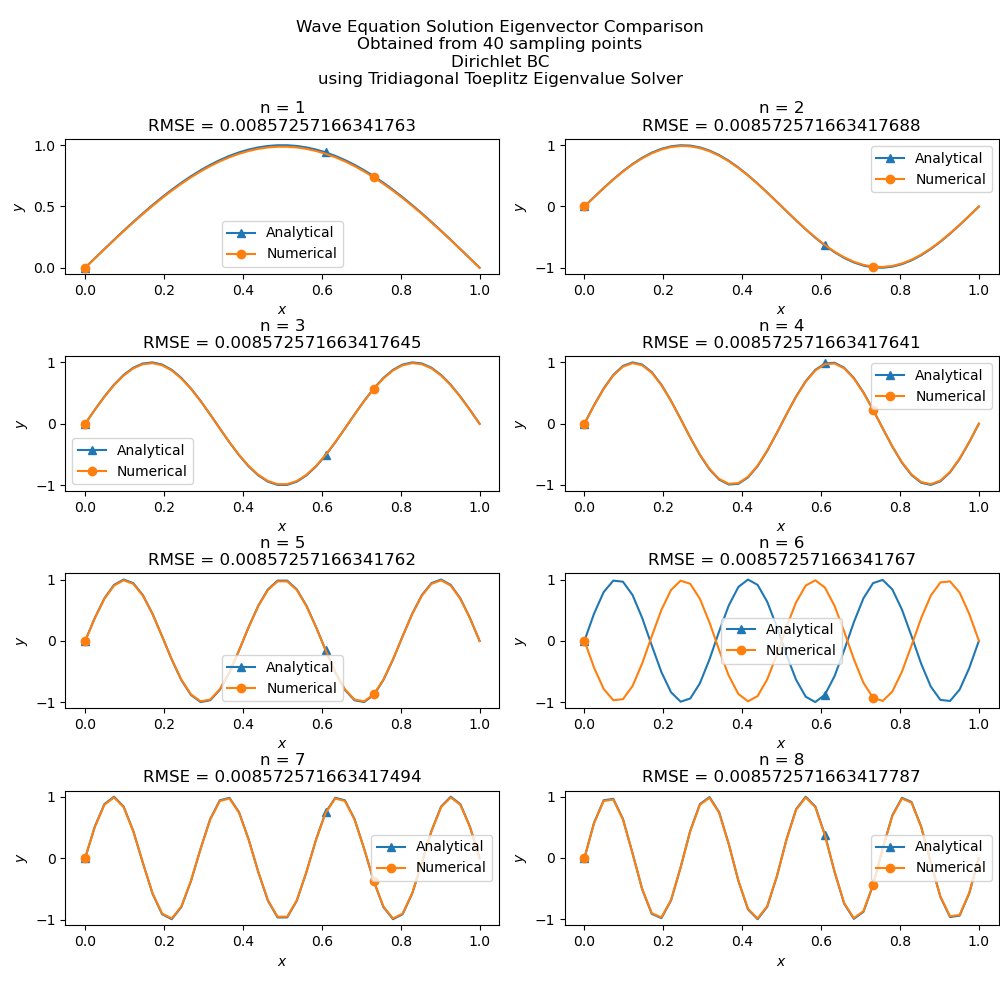
\includegraphics[width=\linewidth]{figures/2_40_Tridiagonal_Toeplitz_Eigenvalue_Solver_d_eigenvector.png}}
\caption{Wave Equation Solution Eigenvectors - 40 Sampling Points - Tridiagonal Toeplitz Eigenvalue Solver - Dirichlet BC}
\label{fig:2_40_Tridiagonal_Toeplitz_Eigenvalue_Solver_d_eigenvector}
\end{figure}
    
\begin{figure}[H]
\centerline{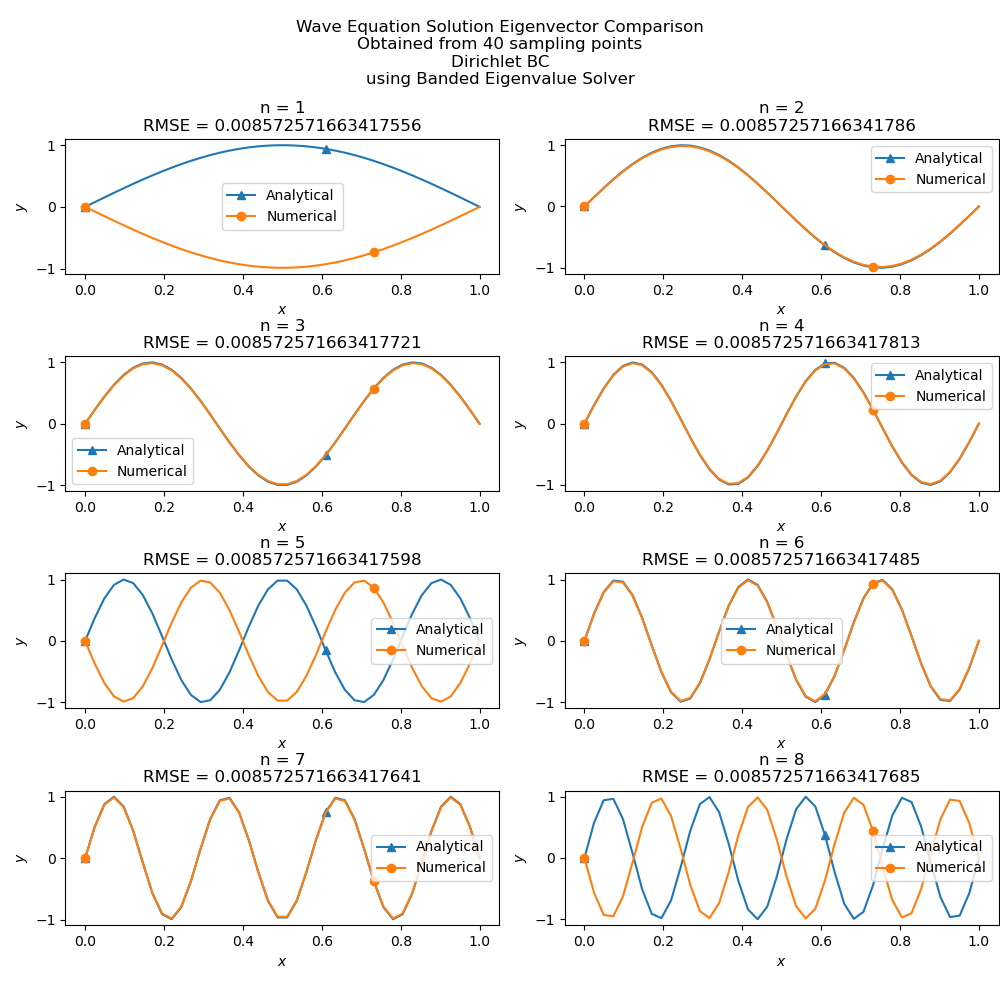
\includegraphics[width=\linewidth]{figures/2_40_Banded_Eigenvalue_Solver_d_eigenvector.png}}
\caption{Wave Equation Solution Eigenvectors - 40 Sampling Points - Banded Eigenvalue Solver - Dirichlet BC}
\label{fig:2_40_Banded_Eigenvalue_Solver_d_eigenvector}
\end{figure}

\begin{figure}[H]
\centerline{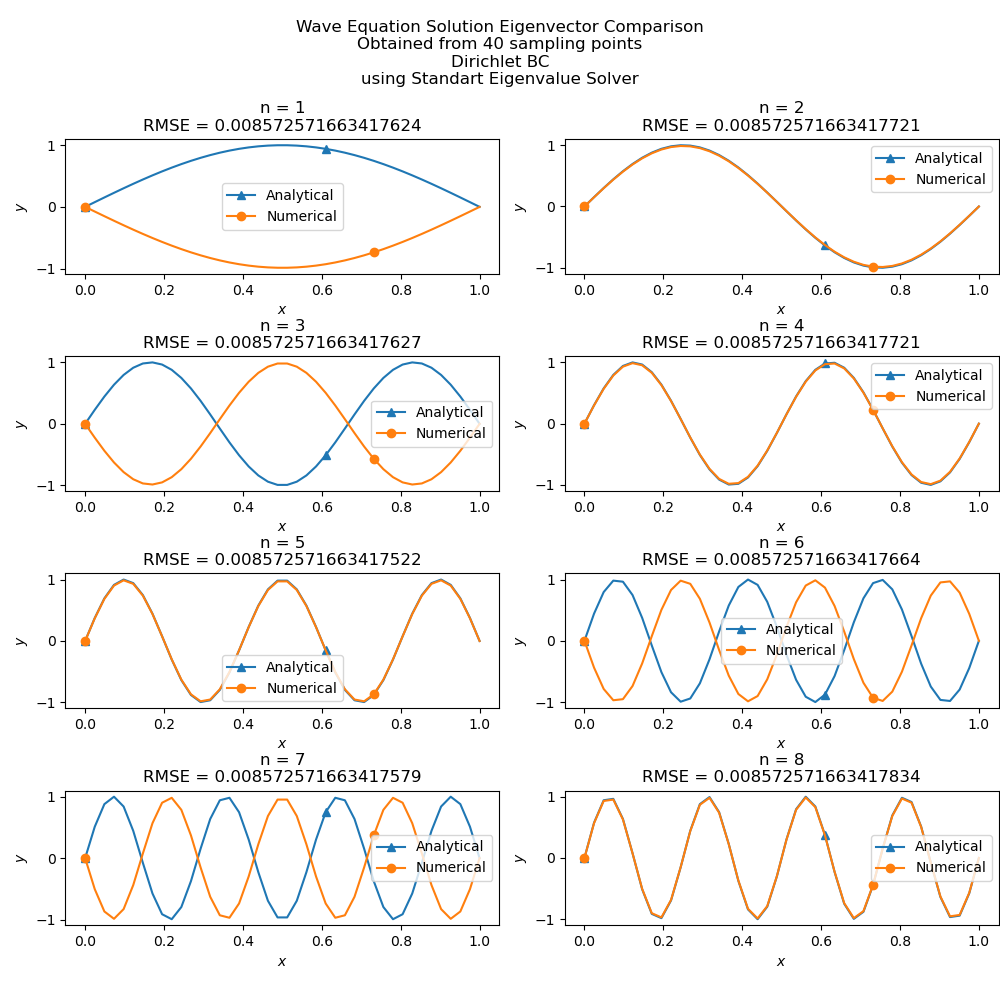
\includegraphics[width=\linewidth]{figures/2_40_Standart_Eigenvalue_Solver_d_eigenvector.png}}
\caption{Wave Equation Solution Eigenvectors - 40 Sampling Points - Tridiagonal Toeplitz Eigenvalue Solver - Dirichlet BC}
\label{fig:2_40_Standart_Eigenvalue_Solver_d_eigenvector}
\end{figure}

\begin{figure}[H]
\centerline{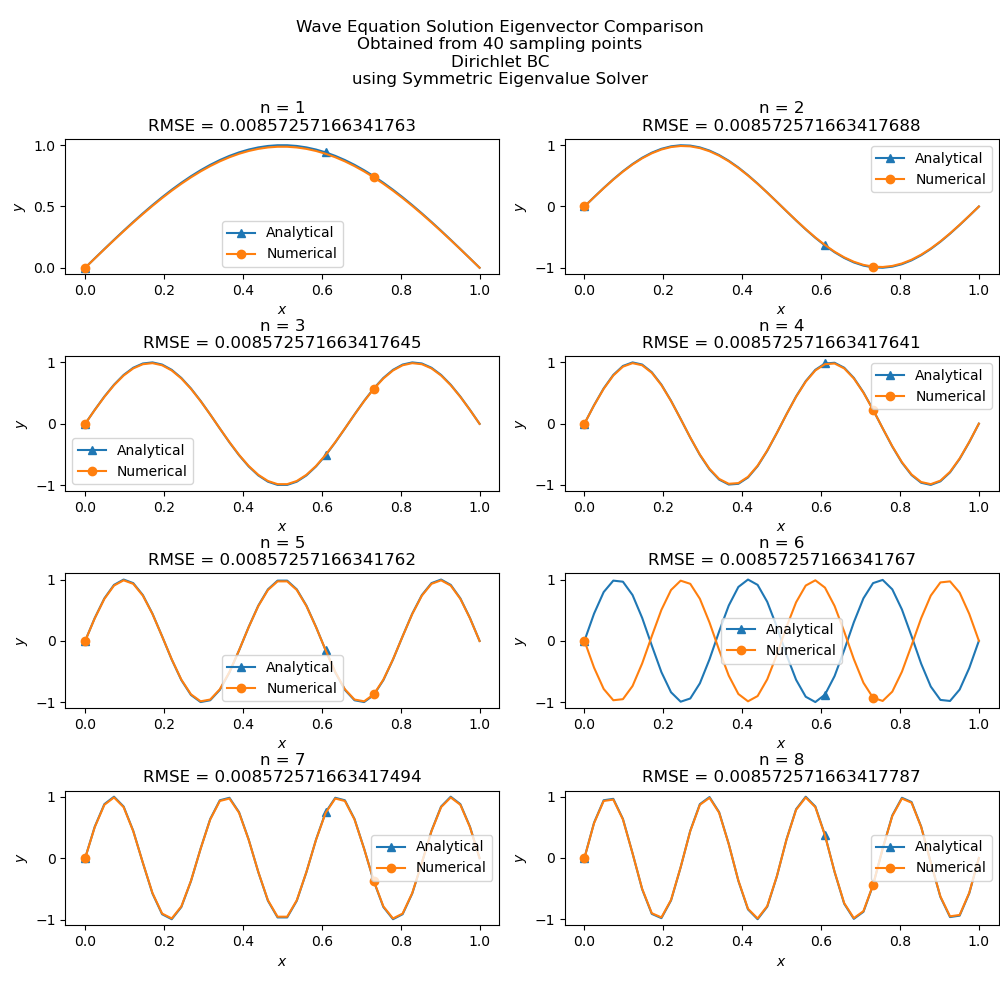
\includegraphics[width=\linewidth]{figures/2_40_Symmetric_Eigenvalue_Solver_d_eigenvector.png}}
\caption{Wave Equation Solution Eigenvectors - 40 Sampling Points - Symmetric Eigenvalue Solver - Dirichlet BC}
\label{fig:2_40_Symmetric_Eigenvalue_Solver_d_eigenvector}
\end{figure}

\begin{figure}[H]
\centerline{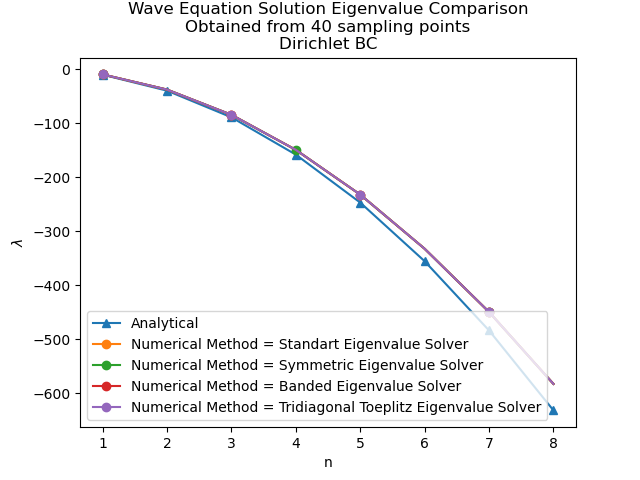
\includegraphics[width=\linewidth]{figures/2_40_d_eigenvalue.png}}
\caption{Wave Equation Solution Eigenvalues - 40 Sampling Points - Dirichlet BC}
\label{fig:2_40_d_eigenvalue}
\end{figure}
    

\subsubsection{Dirichlet Boundary Condition - Eigenvalue Solver Speed Experiment}

\paragraph{} From Figure \ref{fig:3_1024_d_eigen_solver_speed}, it can be easily observed that the different eigenvalue problem solvers yields different elapsation times. For example, it can shown that the \textit{Tridiagonal Toeplitz Eigenvalue Problem Solver} and \textit{Banded Eigenvalue Problem Solver} shows a superiority over the other two methods. One reason for this circumstance might be the fact that \textit{Symmetric Eigenvalue Problem Solver} and \textit{Standart Eigenvalue Problem Solver} takes whole matrix as an input, while \textit{Tridiagonal Toeplitz Eigenvalue Problem Solver} and \textit{Banded Eigenvalue Problem Solver} takes only the main diagonal and the off-diagonal part.
\label{sec:speed}
\begin{figure}[H]
\centerline{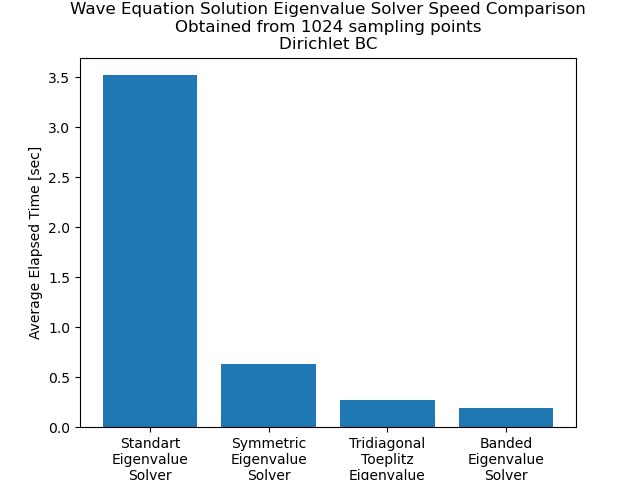
\includegraphics[width=\linewidth]{figures/3_1024_d_eigen_solver_speed.png}}
\caption{Wave Equation Solution Eigenvalue Solver Speed Comparison - 1024 Sampling Points - Dirichlet BC}
\label{fig:3_1024_d_eigen_solver_speed}
\end{figure}

\paragraph{} As an additional note, to be able to demonstrate the real performance of the eigenvalue problem solvers, the number of sampling points are set to $1024$.

\subsubsection{Neumann Boundary Condition - Symmetric Hermitian Matrix Case}

\paragraph{} Observing Figure \ref{fig:4_40_Symmetric_Eigenvalue_Solver_n_eigenvector} and \ref{fig:5_40_Standart_Eigenvalue_Solver_n_eigenvector}, one can easily conclude that the eigenvalue problem solution yields more accurate result when the \textit{Hermitian} matrix is symmetric.

\begin{figure}[H]
\centerline{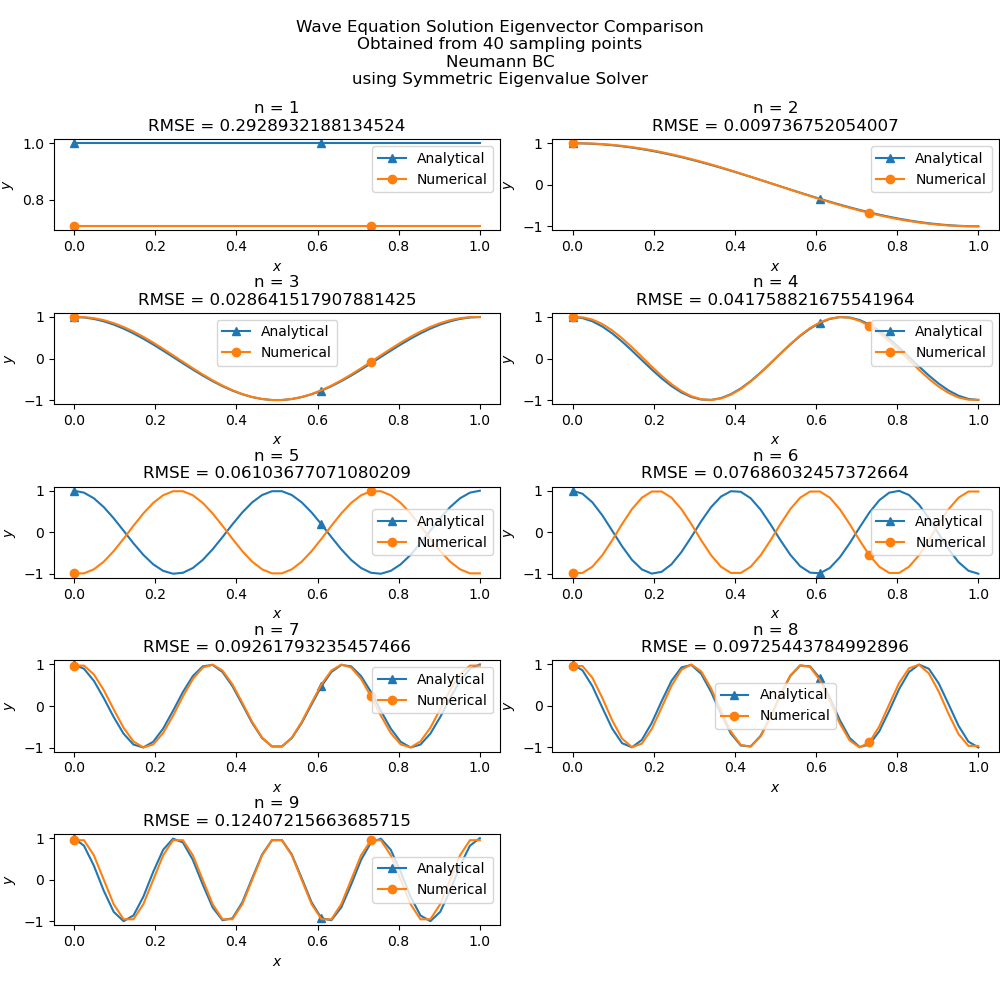
\includegraphics[width=\linewidth]{figures/4_40_Symmetric_Eigenvalue_Solver_n_eigenvector.png}}
\caption{Wave Equation Solution Eigenvectors [Symmetric Hermitian Matrix Case] - 40 Sampling Points - Symmetric Eigenvalue Solver - Neumann BC}
\label{fig:4_40_Symmetric_Eigenvalue_Solver_n_eigenvector}
\end{figure}

\begin{figure}[H]
\centerline{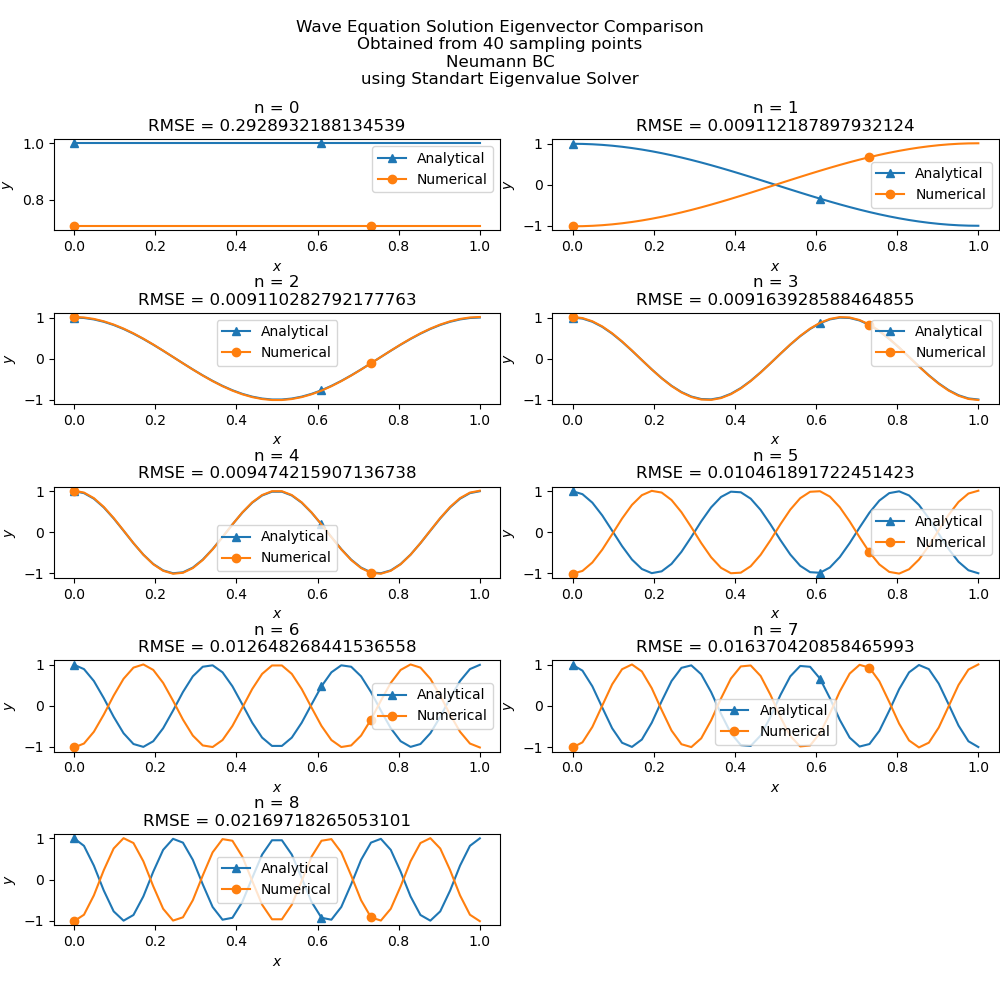
\includegraphics[width=\linewidth]{figures/5_40_Standart_Eigenvalue_Solver_n_eigenvector.png}}
\caption{Wave Equation Solution Eigenvectors [Unsymmetric Hermitian Matrix Case]- 40 Sampling Points - Standart Eigenvalue Solver - Neumann BC}
\label{fig:5_40_Standart_Eigenvalue_Solver_n_eigenvector}
\end{figure}

\begin{figure}[H]
\centerline{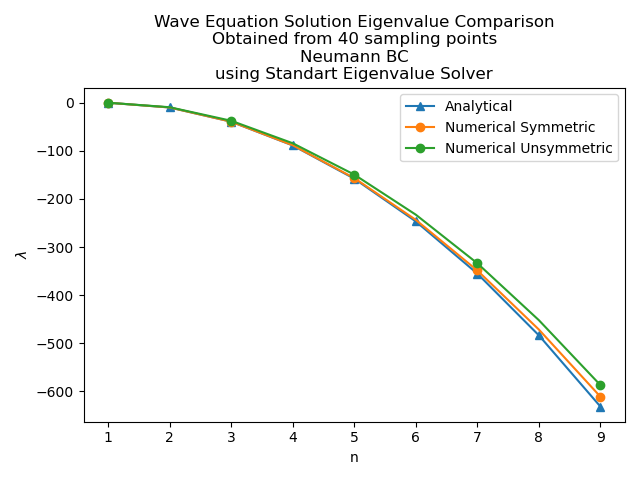
\includegraphics[width=\linewidth]{figures/5_40_Standart_Eigenvalue_Solver_n_eigenvalue.png}}
\caption{Wave Equation Solution Eigenvalues - 40 Sampling Points - Neumann BC}
\label{fig:5_40_Standart_Eigenvalue_Solver_n_eigenvalue}
\end{figure}

\paragraph{} Also, in Figure \ref{fig:5_40_Standart_Eigenvalue_Solver_n_eigenvalue}, the superiority of the symmetric \textit{Hermitian} matrix can be observed. When the \textit{Hermitian} matrix is symmetric, the solution is tended to be more close to the analytical one, which is expected already.

\subsubsection{Periodic Boundary Condition}

\begin{figure}[H]
\centerline{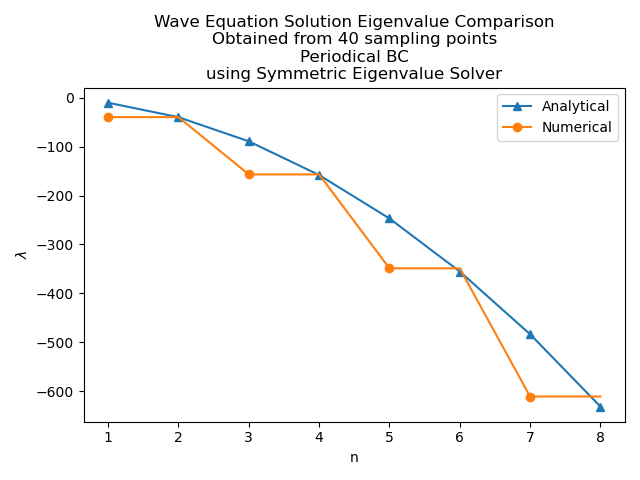
\includegraphics[width=\linewidth]{figures/6_40_Symmetric_Eigenvalue_Solver_p_eigenvalue.png}}
\caption{Wave Equation Solution Eigenvectors - 40 Sampling Points - Symmetric Eigenvalue Solver - Periodic BC}
\label{fig:6_40_Symmetric_Eigenvalue_Solver_p_eigenvalue}
\end{figure}

\begin{figure}[H]
\centerline{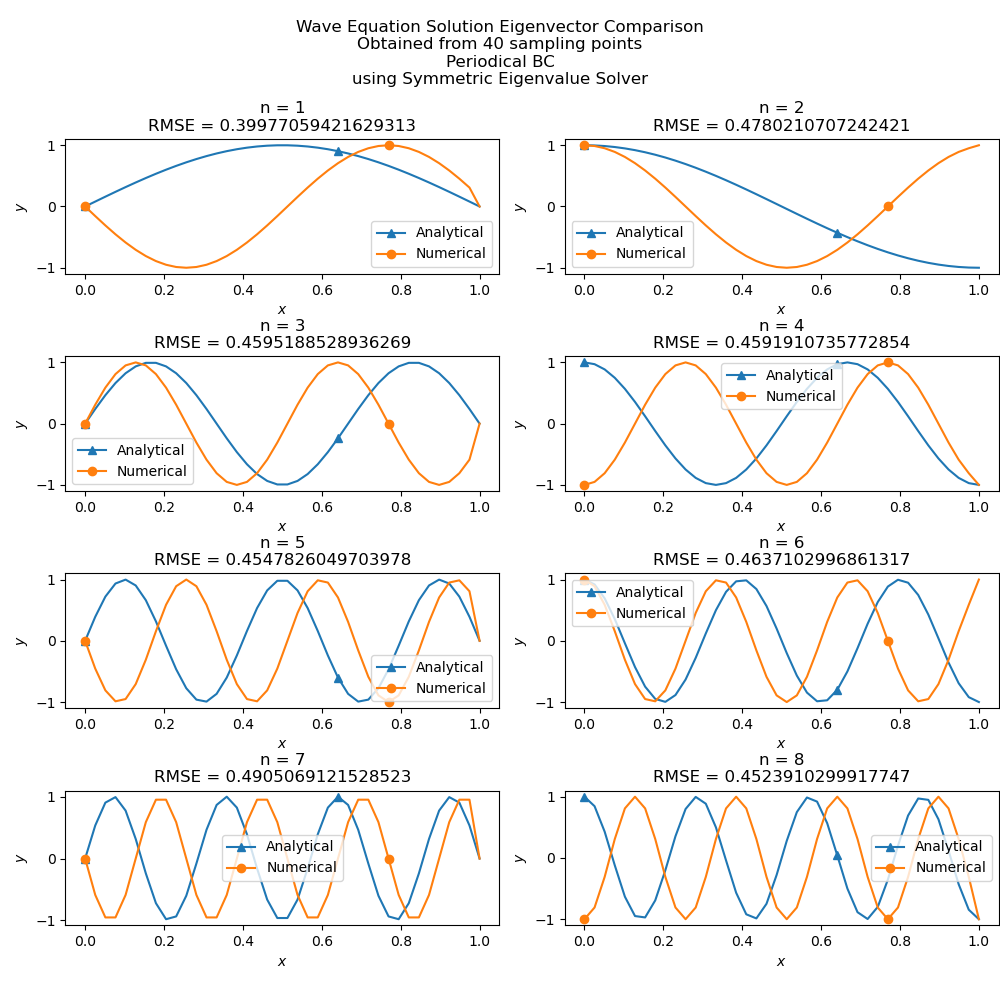
\includegraphics[width=\linewidth]{figures/6_40_Symmetric_Eigenvalue_Solver_p_eigenvector.png}}
\caption{Wave Equation Solution Eigenvalues - 40 Sampling Points - Symmetric Eigenvalue Solver - Periodic BC}
\label{fig:6_40_Symmetric_Eigenvalue_Solver_p_eigenvector}
\end{figure}

\section{Problem XXII}
\subsection{Nondimensionalization of the Half Harmonic Oscillator}
\paragraph{} In the original equation, it is given that:

\begin{equation*}
    \left[-\frac{\hbar^2}{2m} \frac{d^2}{dx^2} + V(x)\right]\psi = E \psi
\end{equation*}

where $V(x) = \frac{1}{2}m\omega^2x^2$ for $x>0$. Therefore, the extension of the equation yields:

\begin{equation*}
    -\frac{\hbar^2}{2m} \frac{d^2 \psi(x)}{dx^2} + V(x)\psi(x) = E \psi(x)
\end{equation*}

\begin{equation*}
    -\frac{\hbar^2}{2m} \frac{d^2 \psi(x)}{dx^2} + \frac{1}{2}m\omega^2x^2\psi(x) = E \psi(x)
\end{equation*}

\paragraph{} In the question, the following set of nondimensionalization process is suggested:

\begin{equation}
    \label{eq:z}
    z = \frac{x}{x_0}
\end{equation}

\begin{equation}
    \label{eq:eps}
    \epsilon = \frac{E}{E_0}
\end{equation}

to yield the following final form:

\begin{equation*}
    \frac{-1}{2}\frac{d^2 \psi}{dz^2} + \frac{1}{2}z^2\psi = \epsilon\psi
\end{equation*}

\paragraph{} Now, it is time apply transformations and find the corresponding $x_0$ and $E_0$ expressions. Due to the \eqref{eq:z}, it can be concluded that:

\begin{equation*}
    \frac{d^2}{dz^2} = \frac{1}{x_0^2} \frac{d^2}{dx^2}
\end{equation*}

\paragraph{} Together with the \eqref{eq:z} and \eqref{eq:eps},the following transformed form can be obtained:

\begin{equation*}
    -\frac{\hbar^2}{2m}\frac{1}{x_0^2}\frac{d^2\psi}{dz^2} + \frac{1}{2}m\omega^2z^2x_0^2\psi = \epsilon E_0 \psi
\end{equation*}

\begin{equation*}
    \left(\frac{\hbar^2}{E_0 m x_0^2}\right)\frac{-1}{2}\frac{d^2\psi}{dz^2} + \left(\frac{m\omega^2x_0^2}{E_0}\right) \frac{1}{2}z^2\psi = \epsilon\psi
\end{equation*}

\paragraph{} Therefore, it can be concluded that:

\begin{equation}
    \label{eq:1}
    \frac{\hbar^2}{E_0 m x_0^2} = 1 \rightarrow  E_0 x_0^2 = \frac{\hbar^2}{m}
\end{equation}

\begin{equation}
    \label{eq:2}
    \frac{m\omega^2x_0^2}{E_0} = 1 \rightarrow \frac{E_0}{x_0^2} = m\omega^2
\end{equation}

\paragraph{}Multiplication of \eqref{eq:1} and \eqref{eq:2} gives that:

\begin{equation}
    \label{eq:3}
   \boxed{ E_0 = \omega\hbar }
\end{equation}

\paragraph{} Plugging \eqref{eq:3} into \eqref{eq:1} or \eqref{eq:2} gives that:

\begin{equation*}
    \boxed{x_0 = \sqrt{\frac{\hbar}{\omega m}}}
\end{equation*}




\subsection{Solution with Shooting Method}

\paragraph{} In Figure \ref{fig:7_eigenfunctions} and \ref{fig:7_eigenvalue}, the solution of the \textit{Half Harmonic Oscillator} can be observed for different $\zeta$ values. 
\begin{figure}[H]
\centerline{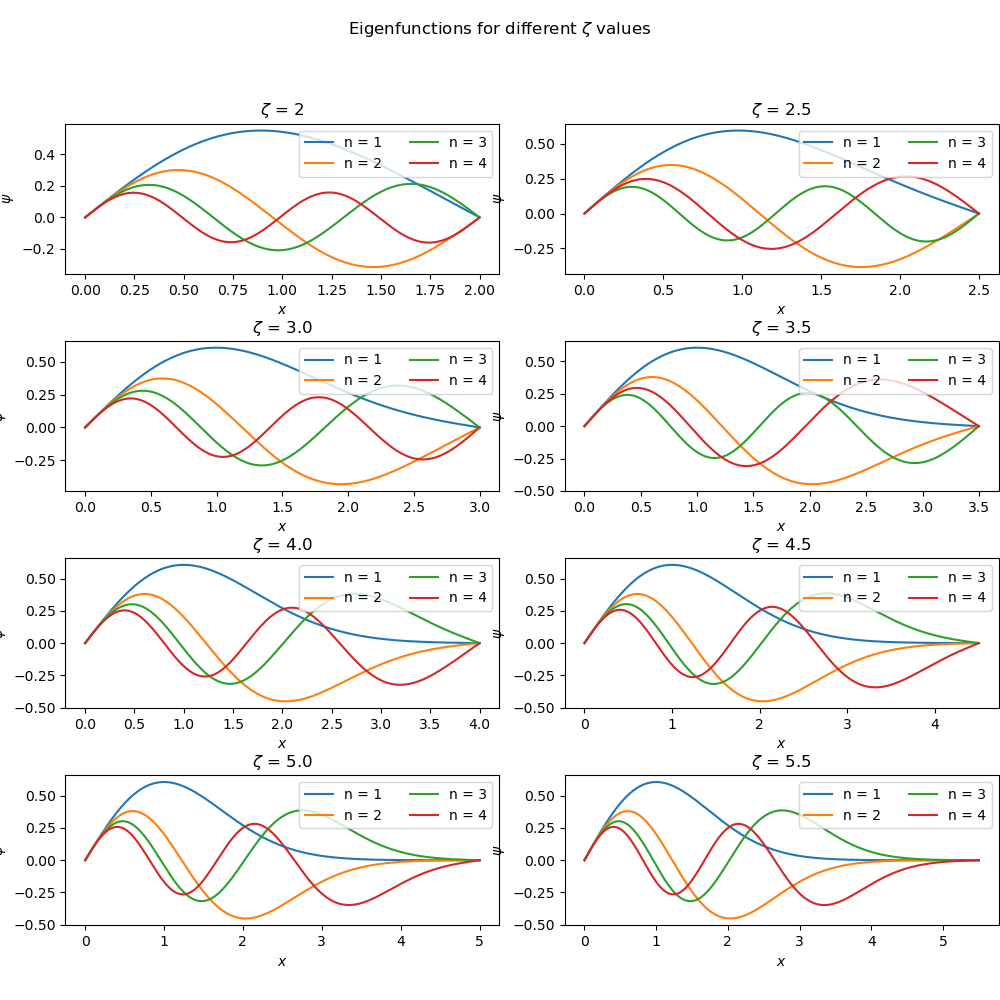
\includegraphics[width=\linewidth]{figures/7_eigenfunctions.png}}
\caption{Eigenfunctions for different $\zeta$ values}
\label{fig:7_eigenfunctions}
\end{figure}

\paragraph{} From Figure \ref{fig:7_eigenfunctions} and Figure \ref{fig:7_eigenvalue}, it can be concluded that the solution does not tend to change so much after a certain point of $\zeta$, i.e. $\zeta = 3.5 - 4.0$.

\paragraph{} From Figure \ref{fig:7_eigenfunctions} and Figure \ref{fig:7_eigenvalue}, it can be easily inferred that the \textit{Shooting Method} is really capable of the approximating the HHO correctly. In the same time, it can be investigated that as $\zeta$ value increases, the rate of change of approximating to the certain value decreases.
\begin{figure}[H]
\centerline{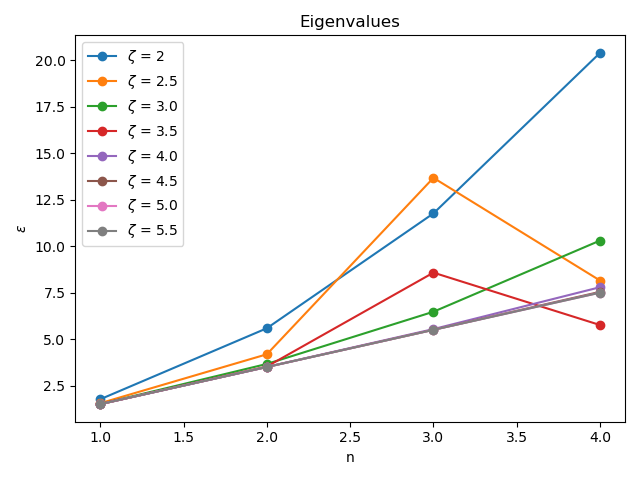
\includegraphics[width=\linewidth]{figures/7_eigenvalue.png}}
\caption{Eigenvalues for different $\zeta$ values}
\label{fig:7_eigenvalue}
\end{figure}

\subsection{Solution with Direct Method}

\paragraph{} From Figure \ref{fig:8_eigenfunctions} and Figure \ref{fig:8_eigenvalue}, it can be observed that the \textit{Direct Method} does not perform well as the \textit{Shooting Method} does. 
\begin{figure}[H]
\centerline{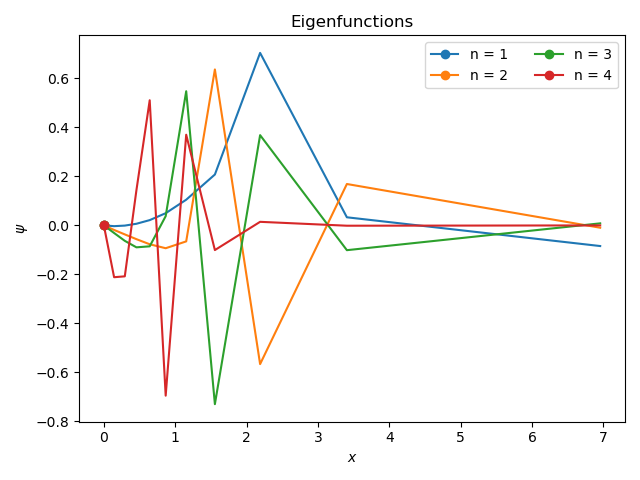
\includegraphics[width=\linewidth]{figures/8_eigenfunctions.png}}
\caption{Eigenfunctions with \textit{Direct Method}}
\label{fig:8_eigenfunctions}
\end{figure}

\begin{figure}[H]
\centerline{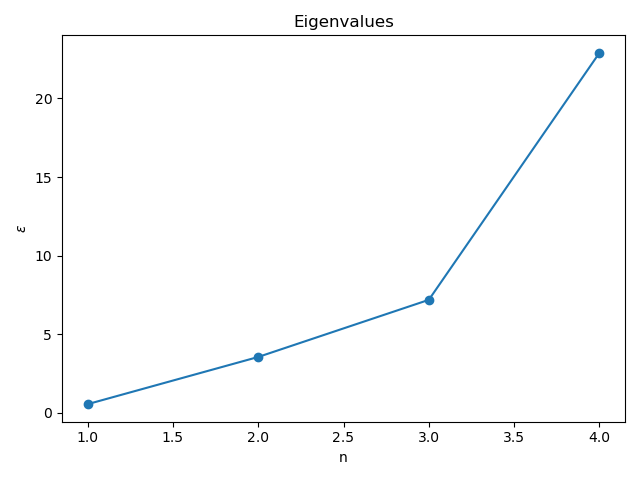
\includegraphics[width=\linewidth]{figures/8_eigenvalue.png}}
\caption{Eigenvalues with \textit{Direct Method}}
\label{fig:8_eigenvalue}
\end{figure}
    
\end{document}



              


